% Detailed Monocular Depth Estimation Timeline
% Two layers: (1) architecture/technology milestones, (2) specific model releases
\documentclass[border=12pt]{standalone}
\usepackage[T1]{fontenc}
\usepackage{tikz}
\usetikzlibrary{arrows.meta,positioning,calc,backgrounds}

% ── Brand Colors ──
\definecolor{garnet}{HTML}{73000A}
\definecolor{rose}{HTML}{CC2E40}
\definecolor{atlantic}{HTML}{466A9F}
\definecolor{congaree}{HTML}{1F414D}
\definecolor{horseshoe}{HTML}{65780B}
\definecolor{grass}{HTML}{CED318}
\definecolor{honeycomb}{HTML}{A49137}
\definecolor{warmgrey}{HTML}{676156}
\definecolor{sandstorm}{HTML}{FFF2E3}
\definecolor{bk90}{HTML}{363636}
\definecolor{bk70}{HTML}{5C5C5C}
\definecolor{bk50}{HTML}{A2A2A2}
\definecolor{bk30}{HTML}{C7C7C7}
\definecolor{bk10}{HTML}{ECECEC}

\begin{document}
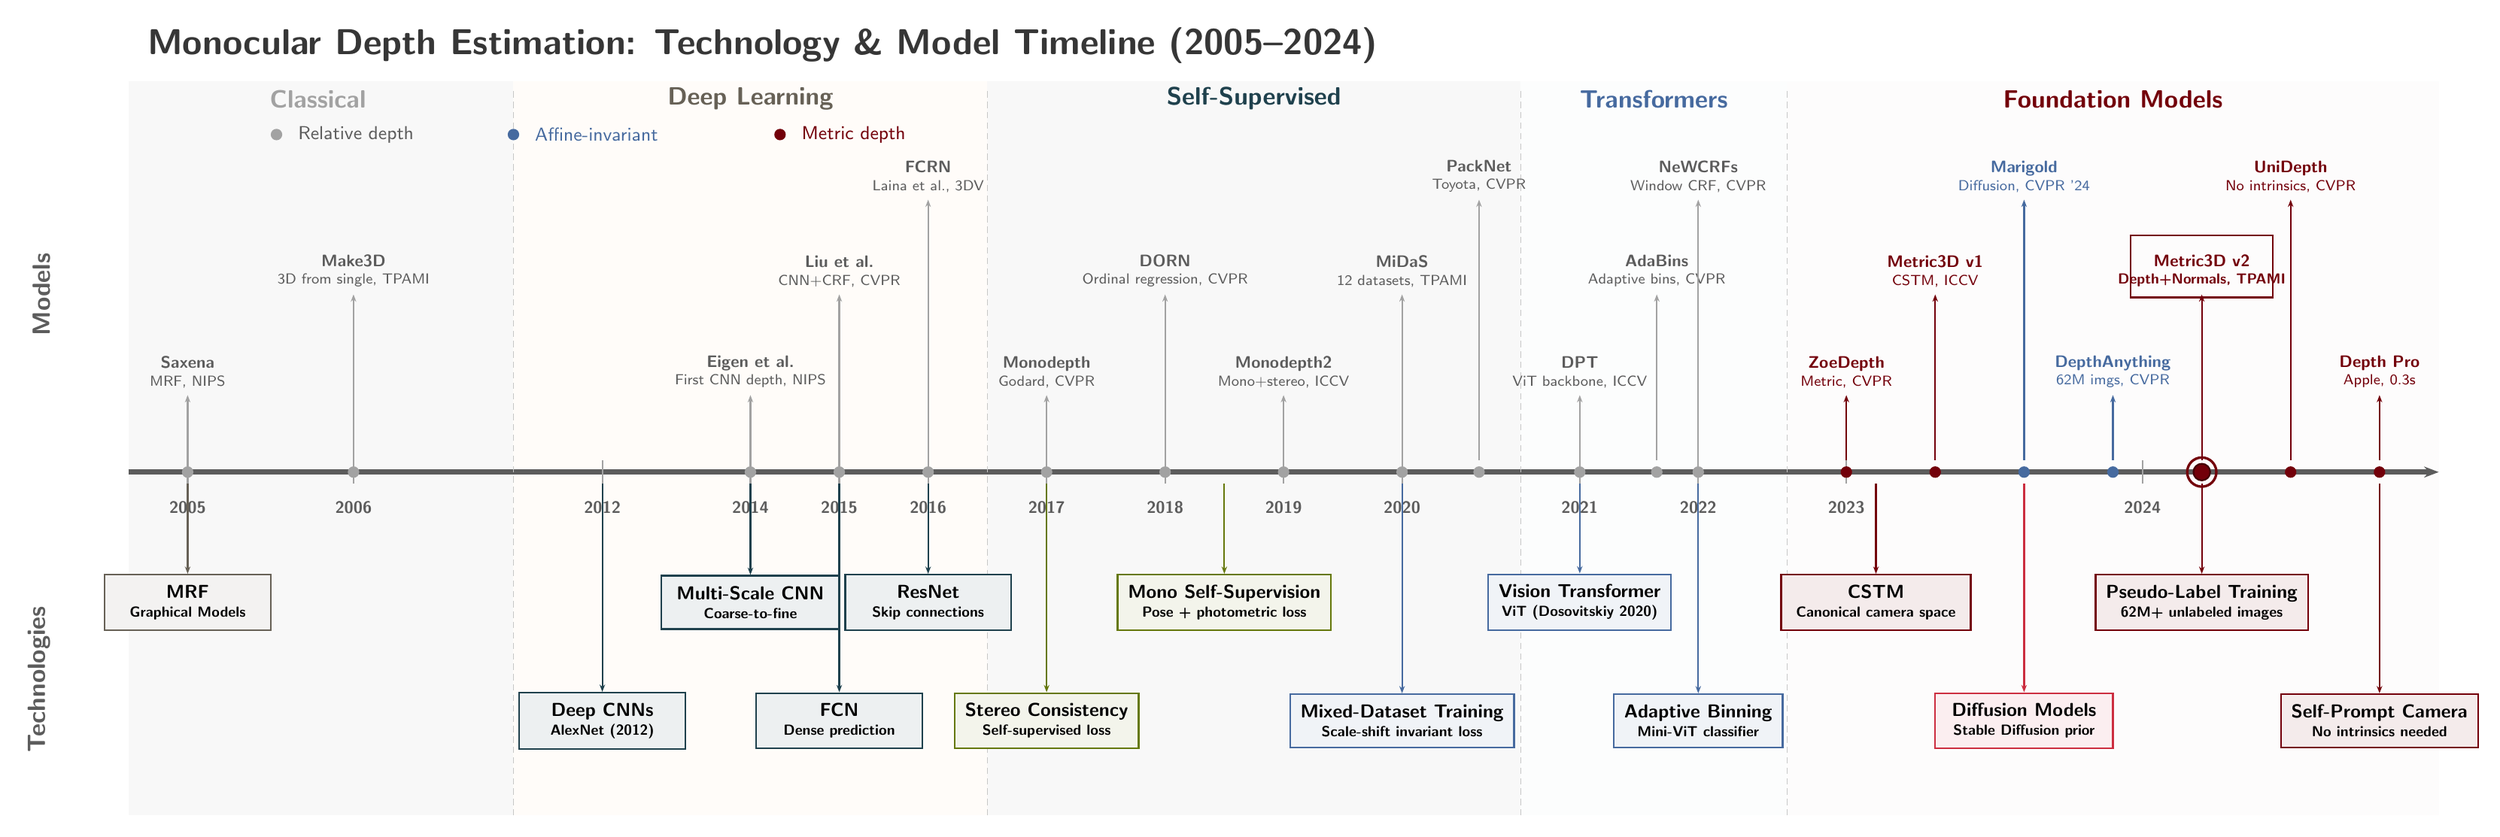
\begin{tikzpicture}[
  % ── Node styles ──
  techbox/.style={
    rectangle, draw=#1, fill=#1!8, thick,
    font=\small\sffamily\bfseries, align=center,
    inner sep=5pt, minimum height=0.9cm, minimum width=2.8cm,
  },
  techbox/.default=bk70,
  modeldot/.style={circle, fill=#1, inner sep=0pt, minimum size=5.5pt},
  bigdot/.style={circle, fill=#1, inner sep=0pt, minimum size=8pt,
                 draw=#1!60!black, line width=0.8pt},
  mlabel/.style={
    font=\footnotesize\sffamily, align=center, color=#1,
  },
  eralabel/.style={
    font=\large\sffamily\bfseries, color=#1,
  },
  stem/.style={thick, color=#1, -{Stealth[length=3.5pt]}},
  tecstem/.style={thick, color=#1, -{Stealth[length=3.5pt]}},
]

  % ══════════════════════════════════════════════════════════════
  % LAYOUT: ~38cm wide, generous spacing
  % Model heights:  h1=1.5, h2=3.2, h3=4.8
  % Tech rows:      t1=-2.2, t2=-4.2
  % ══════════════════════════════════════════════════════════════

  % ── Title ──
  \node[font=\LARGE\sffamily\bfseries, color=bk90, anchor=west]
    at (-0.8, 7.2) {Monocular Depth Estimation: Technology \& Model Timeline (2005--2024)};

  % ── Main timeline arrow ──
  \draw[-{Stealth[length=7pt]}, bk70, line width=2.5pt]
    (-1.0, 0) -- (38.0, 0);

  % ── Year tick marks ──
  \foreach \x/\yr in {
    0.0/2005, 2.8/2006, 7.0/2012, 9.5/2014, 11.0/2015,
    12.5/2016, 14.5/2017, 16.5/2018, 18.5/2019,
    20.5/2020, 23.5/2021, 25.5/2022, 28.0/2023, 33.0/2024%
  } {
    \draw[bk50, thick] (\x, -0.2) -- (\x, 0.2);
    \node[font=\footnotesize\sffamily\bfseries, color=bk70, below=5pt]
      at (\x, -0.2) {\yr};
  }

  % ── Era background bands ──
  \begin{scope}[on background layer]
    \fill[bk10, opacity=0.35] (-1.0, -5.8) rectangle (5.5, 6.6);
    \fill[sandstorm, opacity=0.2] (5.5, -5.8) rectangle (13.5, 6.6);
    \fill[bk10, opacity=0.35] (13.5, -5.8) rectangle (22.5, 6.6);
    \fill[atlantic!5, opacity=0.35] (22.5, -5.8) rectangle (27.0, 6.6);
    \fill[garnet!4, opacity=0.35] (27.0, -5.8) rectangle (38.0, 6.6);
  \end{scope}

  % ── Era labels ──
  \node[eralabel=bk50] at (2.2, 6.3) {Classical};
  \node[eralabel=warmgrey] at (9.5, 6.3) {Deep Learning};
  \node[eralabel=congaree] at (18.0, 6.3) {Self-Supervised};
  \node[eralabel=atlantic] at (24.75, 6.3) {Transformers};
  \node[eralabel=garnet] at (32.5, 6.3) {Foundation Models};

  % Era dividers
  \draw[bk30, densely dashed] (5.5, -5.8) -- (5.5, 6.5);
  \draw[bk30, densely dashed] (13.5, -5.8) -- (13.5, 6.5);
  \draw[bk30, densely dashed] (22.5, -5.8) -- (22.5, 6.5);
  \draw[bk30, densely dashed] (27.0, -5.8) -- (27.0, 6.5);

  % ── Layer labels ──
  \node[font=\large\sffamily\bfseries, color=bk70, rotate=90,
        anchor=south] at (-2.2, 3.0) {Models};
  \node[font=\large\sffamily\bfseries, color=bk70, rotate=90,
        anchor=south] at (-2.2, -3.5) {Technologies};

  % ── Legend ──
  \node[modeldot=bk50] at (1.5, 5.7) {};
  \node[font=\small\sffamily, color=bk70, right=4pt] at (1.6, 5.7)
    {Relative depth};
  \node[modeldot=atlantic] at (5.5, 5.7) {};
  \node[font=\small\sffamily, color=atlantic, right=4pt] at (5.6, 5.7)
    {Affine-invariant};
  \node[modeldot=garnet] at (10.0, 5.7) {};
  \node[font=\small\sffamily, color=garnet, right=4pt] at (10.1, 5.7)
    {Metric depth};

  % ══════════════════════════════════════════════════════════════
  % LAYER 1 (BELOW): Technologies & Architectures
  % Row 1: y=-2.2   Row 2: y=-4.2
  % ══════════════════════════════════════════════════════════════

  % ── MRF / Graphical Models (2005) ── row 1
  \node[techbox=warmgrey] (mrf) at (0.0, -2.2) {
    MRF\\[-2pt]{\scriptsize Graphical Models}
  };
  \draw[tecstem=warmgrey] (0.0, -0.2) -- (mrf.north);

  % ── Deep CNNs / AlexNet (2012) ── row 2
  \node[techbox=congaree] (cnn) at (7.0, -4.2) {
    Deep CNNs\\[-2pt]{\scriptsize AlexNet (2012)}
  };
  \draw[tecstem=congaree] (7.0, -0.2) -- (cnn.north);

  % ── Multi-Scale CNN (2014) ── row 1
  \node[techbox=congaree, minimum width=3.0cm] (mscnn) at (9.5, -2.2) {
    Multi-Scale CNN\\[-2pt]{\scriptsize Coarse-to-fine}
  };
  \draw[tecstem=congaree] (9.5, -0.2) -- (mscnn.north);

  % ── FCN (2015) ── row 2
  \node[techbox=congaree] (fcn) at (11.0, -4.2) {
    FCN\\[-2pt]{\scriptsize Dense prediction}
  };
  \draw[tecstem=congaree] (11.0, -0.2) -- (fcn.north);

  % ── ResNet (2016) ── row 1
  \node[techbox=congaree] (resnet) at (12.5, -2.2) {
    ResNet\\[-2pt]{\scriptsize Skip connections}
  };
  \draw[tecstem=congaree] (12.5, -0.2) -- (resnet.north);

  % ── Stereo Consistency (2017) ── row 2
  \node[techbox=horseshoe, minimum width=3.0cm] (stereo) at (14.5, -4.2) {
    Stereo Consistency\\[-2pt]{\scriptsize Self-supervised loss}
  };
  \draw[tecstem=horseshoe] (14.5, -0.2) -- (stereo.north);

  % ── Mono Self-Supervision (2018-19) ── row 1
  \node[techbox=horseshoe, minimum width=3.2cm] (monossl) at (17.5, -2.2) {
    Mono Self-Supervision\\[-2pt]{\scriptsize Pose + photometric loss}
  };
  \draw[tecstem=horseshoe] (17.5, -0.2) -- (monossl.north);

  % ── Mixed-Dataset Training (2020) ── row 2
  \node[techbox=atlantic, minimum width=3.2cm] (mixdata) at (20.5, -4.2) {
    Mixed-Dataset Training\\[-2pt]{\scriptsize Scale-shift invariant loss}
  };
  \draw[tecstem=atlantic] (20.5, -0.2) -- (mixdata.north);

  % ── Vision Transformer (2021) ── row 1
  \node[techbox=atlantic, minimum width=3.0cm] (vit) at (23.5, -2.2) {
    Vision Transformer\\[-2pt]{\scriptsize ViT (Dosovitskiy 2020)}
  };
  \draw[tecstem=atlantic] (23.5, -0.2) -- (vit.north);

  % ── Adaptive Binning (2021) ── row 2
  \node[techbox=atlantic] (adabin) at (25.5, -4.2) {
    Adaptive Binning\\[-2pt]{\scriptsize Mini-ViT classifier}
  };
  \draw[tecstem=atlantic] (25.5, -0.2) -- (adabin.north);

  % ── CSTM (2023) ── row 1
  \node[techbox=garnet, minimum width=3.2cm] (cstm) at (28.5, -2.2) {
    CSTM\\[-2pt]{\scriptsize Canonical camera space}
  };
  \draw[tecstem=garnet] (28.5, -0.2) -- (cstm.north);

  % ── Diffusion Models (2023) ── row 2
  \node[techbox=rose, minimum width=3.0cm] (diffusion) at (31.0, -4.2) {
    Diffusion Models\\[-2pt]{\scriptsize Stable Diffusion prior}
  };
  \draw[tecstem=rose] (31.0, -0.2) -- (diffusion.north);

  % ── Pseudo-Label Training (2024) ── row 1
  \node[techbox=garnet, minimum width=3.2cm] (pseudo) at (34.0, -2.2) {
    Pseudo-Label Training\\[-2pt]{\scriptsize 62M+ unlabeled images}
  };
  \draw[tecstem=garnet] (34.0, -0.2) -- (pseudo.north);

  % ── Self-Promptable Camera (2024) ── row 2
  \node[techbox=garnet, minimum width=3.0cm] (selfprompt) at (37.0, -4.2) {
    Self-Prompt Camera\\[-2pt]{\scriptsize No intrinsics needed}
  };
  \draw[tecstem=garnet] (37.0, -0.2) -- (selfprompt.north);

  % ══════════════════════════════════════════════════════════════
  % LAYER 2 (ABOVE): Model Releases
  % Heights: h1=1.5, h2=3.2, h3=4.8
  % ══════════════════════════════════════════════════════════════

  % ────────────────── Classical ──────────────────

  % Saxena 2005 — h1
  \node[modeldot=bk50] at (0.0, 0) {};
  \draw[stem=bk50] (0.0, 0.2) -- (0.0, 1.3);
  \node[mlabel=bk70, above=0pt] at (0.0, 1.3) {
    \textbf{Saxena}\\[-1pt]{\scriptsize MRF, NIPS}
  };

  % Make3D 2006 — h2
  \node[modeldot=bk50] at (2.8, 0) {};
  \draw[stem=bk50] (2.8, 0.2) -- (2.8, 3.0);
  \node[mlabel=bk70, above=0pt] at (2.8, 3.0) {
    \textbf{Make3D}\\[-1pt]{\scriptsize 3D from single, TPAMI}
  };

  % ────────────────── Deep Learning ──────────────────

  % Eigen 2014 — h1
  \node[modeldot=bk50] at (9.5, 0) {};
  \draw[stem=bk50] (9.5, 0.2) -- (9.5, 1.3);
  \node[mlabel=bk70, above=0pt] at (9.5, 1.3) {
    \textbf{Eigen et al.}\\[-1pt]{\scriptsize First CNN depth, NIPS}
  };

  % Liu 2015 — h2
  \node[modeldot=bk50] at (11.0, 0) {};
  \draw[stem=bk50] (11.0, 0.2) -- (11.0, 3.0);
  \node[mlabel=bk70, above=0pt] at (11.0, 3.0) {
    \textbf{Liu et al.}\\[-1pt]{\scriptsize CNN+CRF, CVPR}
  };

  % FCRN 2016 — h3
  \node[modeldot=bk50] at (12.5, 0) {};
  \draw[stem=bk50] (12.5, 0.2) -- (12.5, 4.6);
  \node[mlabel=bk70, above=0pt] at (12.5, 4.6) {
    \textbf{FCRN}\\[-1pt]{\scriptsize Laina et al., 3DV}
  };

  % ────────────────── Self-Supervised ──────────────────

  % Monodepth 2017 — h1
  \node[modeldot=bk50] at (14.5, 0) {};
  \draw[stem=bk50] (14.5, 0.2) -- (14.5, 1.3);
  \node[mlabel=bk70, above=0pt] at (14.5, 1.3) {
    \textbf{Monodepth}\\[-1pt]{\scriptsize Godard, CVPR}
  };

  % DORN 2018 — h2
  \node[modeldot=bk50] at (16.5, 0) {};
  \draw[stem=bk50] (16.5, 0.2) -- (16.5, 3.0);
  \node[mlabel=bk70, above=0pt] at (16.5, 3.0) {
    \textbf{DORN}\\[-1pt]{\scriptsize Ordinal regression, CVPR}
  };

  % Monodepth2 2019 — h1
  \node[modeldot=bk50] at (18.5, 0) {};
  \draw[stem=bk50] (18.5, 0.2) -- (18.5, 1.3);
  \node[mlabel=bk70, above=0pt] at (18.5, 1.3) {
    \textbf{Monodepth2}\\[-1pt]{\scriptsize Mono+stereo, ICCV}
  };

  % MiDaS 2020 — h2
  \node[modeldot=bk50] at (20.5, 0) {};
  \draw[stem=bk50] (20.5, 0.2) -- (20.5, 3.0);
  \node[mlabel=bk70, above=0pt] at (20.5, 3.0) {
    \textbf{MiDaS}\\[-1pt]{\scriptsize 12 datasets, TPAMI}
  };

  % PackNet 2020 — h3
  \node[modeldot=bk50] at (21.8, 0) {};
  \draw[stem=bk50] (21.8, 0.2) -- (21.8, 4.6);
  \node[mlabel=bk70, above=0pt] at (21.8, 4.6) {
    \textbf{PackNet}\\[-1pt]{\scriptsize Toyota, CVPR}
  };

  % ────────────────── Transformers ──────────────────

  % DPT 2021 — h1
  \node[modeldot=bk50] at (23.5, 0) {};
  \draw[stem=bk50] (23.5, 0.2) -- (23.5, 1.3);
  \node[mlabel=bk70, above=0pt] at (23.5, 1.3) {
    \textbf{DPT}\\[-1pt]{\scriptsize ViT backbone, ICCV}
  };

  % AdaBins 2021 — h2
  \node[modeldot=bk50] at (24.8, 0) {};
  \draw[stem=bk50] (24.8, 0.2) -- (24.8, 3.0);
  \node[mlabel=bk70, above=0pt] at (24.8, 3.0) {
    \textbf{AdaBins}\\[-1pt]{\scriptsize Adaptive bins, CVPR}
  };

  % NeWCRFs 2022 — h3
  \node[modeldot=bk50] at (25.5, 0) {};
  \draw[stem=bk50] (25.5, 0.2) -- (25.5, 4.6);
  \node[mlabel=bk70, above=0pt] at (25.5, 4.6) {
    \textbf{NeWCRFs}\\[-1pt]{\scriptsize Window CRF, CVPR}
  };

  % ────────────────── Foundation Models ──────────────────

  % ZoeDepth 2023 — h1 (metric)
  \node[modeldot=garnet] at (28.0, 0) {};
  \draw[stem=garnet] (28.0, 0.2) -- (28.0, 1.3);
  \node[mlabel=garnet, above=0pt] at (28.0, 1.3) {
    \textbf{ZoeDepth}\\[-1pt]{\scriptsize Metric, CVPR}
  };

  % Metric3D v1 2023 — h2 (metric)
  \node[modeldot=garnet] at (29.5, 0) {};
  \draw[stem=garnet] (29.5, 0.2) -- (29.5, 3.0);
  \node[mlabel=garnet, above=0pt] at (29.5, 3.0) {
    \textbf{Metric3D v1}\\[-1pt]{\scriptsize CSTM, ICCV}
  };

  % Marigold 2023 — h3 (affine)
  \node[modeldot=atlantic] at (31.0, 0) {};
  \draw[stem=atlantic] (31.0, 0.2) -- (31.0, 4.6);
  \node[mlabel=atlantic, above=0pt] at (31.0, 4.6) {
    \textbf{Marigold}\\[-1pt]{\scriptsize Diffusion, CVPR '24}
  };

  % DepthAnything 2024 — h1 (affine)
  \node[modeldot=atlantic] at (32.5, 0) {};
  \draw[stem=atlantic] (32.5, 0.2) -- (32.5, 1.3);
  \node[mlabel=atlantic, above=0pt] at (32.5, 1.3) {
    \textbf{DepthAnything}\\[-1pt]{\scriptsize 62M imgs, CVPR}
  };

  % Metric3D v2 2024 — h2 (metric, HIGHLIGHTED)
  \node[bigdot=garnet] at (34.0, 0) {};
  \draw[garnet, very thick] (34.0, 0) circle (7pt);
  \draw[stem=garnet] (34.0, 0.2) -- (34.0, 3.0);
  \node[mlabel=garnet, above=0pt,
        font=\footnotesize\sffamily\bfseries] at (34.0, 3.0) {
    \textbf{Metric3D v2}\\[-1pt]{\scriptsize Depth+Normals, TPAMI}
  };
  % Highlight box
  \draw[garnet, thick] ($(34.0, 3.15) + (-1.2, -0.2)$)
    rectangle ($(34.0, 3.15) + (1.2, 0.85)$);

  % UniDepth 2024 — h3 (metric)
  \node[modeldot=garnet] at (35.5, 0) {};
  \draw[stem=garnet] (35.5, 0.2) -- (35.5, 4.6);
  \node[mlabel=garnet, above=0pt] at (35.5, 4.6) {
    \textbf{UniDepth}\\[-1pt]{\scriptsize No intrinsics, CVPR}
  };

  % Depth Pro 2024 — h1 (metric)
  \node[modeldot=garnet] at (37.0, 0) {};
  \draw[stem=garnet] (37.0, 0.2) -- (37.0, 1.3);
  \node[mlabel=garnet, above=0pt] at (37.0, 1.3) {
    \textbf{Depth Pro}\\[-1pt]{\scriptsize Apple, 0.3s}
  };

\end{tikzpicture}
\end{document}
